As introduced in \Cref{sec:back:dt:dte}, the concept of \acl{DTE} has been proposed to address the need of representing application scenarios that involve multiple \acp{PA} that are interconnected and interdependent.

While conceptual models lay out a foundation for \acp{DTE}, they leave an operational gap towards their practical implementation.
%
Additionally, real-world deployments are, in many cases, not greenfield: the integration of existing \ac{DT} infrastructures is not only desirable but often essential. 
%
Therefore, arguably, \acp{DTE} implementations must account for the challenges that arise when integrating \acp{DT} of different entities, belonging to possibly different stakeholders, and potentially built using different technologies.

In this chapter, the concept of \aclp{DTE} is further elaborated by providing a characterization in terms of their functionalities and the architectural patterns that emerge from the analysis of existing practice. 
%
This characterization will serve as a foundation for the discussion on the research challenges in the context of practical realizing \acp{DTE} which are addressed in this thesis in the following chapters.



%======================================================
\section{Characterizing \aclp{DTE}}
\label{sec:dte:dte:ecosystems}
%======================================================

\acp{DTE} emerge as a natural evolution of the \ac{DT} concept, driven by the need of breaking out of the silos of individual \acp{DT} to better represent the interactions that occur in the physical world among different \acp{PA} which can rarely be considered completely in isolation. 

This is particularly relevant when taking the perspective of using \acp{DT} as system-wide abstractions to design \ac{CPS}. 
%
For the scope of this thesis, the following definition of \acl{DTE} is adopted:

\begin{quotation}
    A \acl{DTE} is a dynamic set of \aclp{DT}, each modeling a \acl{PA}, whose meaningful relationships within a target context make it valuable to consider their collective evolution to accurately represent the mirrored portion of the physical world.
\end{quotation}

This definition highlights three key aspects of \aclp{DTE}:
\begin{itemize}
    \item \textbf{Dynamic set of \aclp{DT}}: \acp{DTE} are not static constructs; they can evolve over time as new \acp{DT} are added or removed, reflecting changes in the physical environment or system requirements.
    
    \item \textbf{Meaningful relationships}: The interactions and dependencies among the constituent \acp{DT} are crucial. These relationships can be functional, spatial, temporal, or based on data exchange, and they define how the \acp{DT} influence each other within the ecosystem.
    
    \item \textbf{Collective evolution}: The value of a \ac{DTE} lies in its ability to represent the collective behavior of its constituent \acp{DT}. This holistic view enables new forms of interactions that support processes that consider the interdependencies among multiple \acp{PA}.
\end{itemize}

From a functional perspective, there are two roles that \acp{DTE} users can assume: 

\paragraph{\ac{DTE} Managers} may need to oversee the creation and evolution of the ecosystem. 
%
From such management perspective, 
being a \emph{dynamic} set of \acp{DT}, members could join or leave the ecosystem at any time for different reasons.
These include the \acp{PA} lifecycle (e.g., decommissioning) or application-specific inclusion criteria adopted when modeling the ecosystem (e.g., entering or exiting a geographical area).
%
To support this dynamism, \acp{DTE} should provide operations to \emph{add} and \emph{remove} \acp{DT}.
These can be public or restricted to administrators, and invocations can be either manual or automatically triggered by monitoring processes (or the \acp{DT} themselves) when detecting relevant changes in the physical environment.
%
A consequence of this dynamicity is the need to easily \emph{discover} which \acp{DT} are part of the ecosystem.
\acp{DTE} may hold an index of all (currently) registered \acp{DT}, each \emph{uniquely identified} and described with metadata to support fine-grained discovery.
%
A key piece of information to store is the mirrored \ac{PA} identifier, allowing tracking of both the digital and physical components of the ecosystem.
Since multiple \acp{DT} may represent the same \ac{PA} for different purposes, this information becomes especially valuable.
Moreover, to keep track of a \ac{DT} evolution, it should be possible to \emph{update} metadata over time.


\paragraph{\ac{DTE} Consumers} represent either human users, applications, or intelligent agents which may be interested in observing the state of the registered \acp{DT} and exploiting their services.
%
An ecosystem should then offer functionalities to access individual \acp{DT} and ecosystem-wide services.
This includes the ability to retrieve the current \emph{representation} of the state of all \acp{DT} and their relationship at a given time.
%
As the representation of the whole ecosystem could be large and difficult to navigate, consumers should also be able to \emph{query} the ecosystem, enabling them to selectively access and aggregate relevant data across multiple \acp{DT}.
%
This supports the derivation of insights that would not be easily discovered by accessing each \ac{DT} individually.
%
Given the dynamic nature of \acp{DT} continuously updating their representation of the corresponding \acp{PA}, \acp{DTE} should support \emph{observation} patterns---possibly selectively through continuous queries~\cite{babu2001sigmod}---to track changes of \acp{DT} and of the whole ecosystem over time.
Finally, \emph{navigation} by following \ac{DT} relationships is a fundamental feature of \acp{DTE}, complementing the other interaction patterns.
%
This allows users to explore and discover information progressively.
Moreover, relationships may cross ecosystem boundaries, offering paths to discover related \acp{DTE}.

\begin{table}
\centering
\begin{adjustbox}{width=\textwidth}
\begin{threeparttable}[b]
 \begin{tabular}{l|c|c|c|c}
    \toprule
    \midrule
    \textbf{} & \textbf{\makecell{Azure Digital\\Twins}} & \textbf{\makecell{Amazon IoT\\TwinMaker}} & \textbf{\makecell{Eclipse\\Ditto}} & \textbf{\makecell{Twinbase\\\cite{Autiosalo_Siegel_Tammi_2021}}} \\
    \hline
    \hline
    \textit{\makecell{\ac{DT} Add/Remove}} & HTTP API & HTTP API & HTTP API & \makecell{GitHub API}  \\
    \hline
    \textit{\makecell{DT Relationships}} & Yes & No\tnote{a} & No & Yes \\
    \hline
    \textit{\makecell{\ac{DT} Description}} & \makecell{DTDL\\+ JSON} & No\tnote{a} & \makecell{WoT TD\\+ Ditto Thing} & JSON/YAML \\
    \hline
    \textit{\makecell{Self-described API}} & No & No  & WoT TD & No \\
    \hline
    \textit{\makecell{Query Support}} & \makecell{ADT Query\\Language\tnote{b}} & \makecell{PartiQL\tnote{c}} & No & No \\
    \hline

    \textit{\makecell{Observe \acp{DT}}} & \makecell{Req. Integration} & \makecell{Req. Integration} & \makecell{WebSocket} & No  \\
    \hline
    \bottomrule
    \end{tabular}
\begin{tablenotes}
\item [a] Amazon IoT TwinMaker uses \emph{entities} as the main concept, defined as parts of a DT so there is no clear description of a DT
\item [b] \url{https://learn.microsoft.com/en-us/azure/digital-twins/concepts-query-language}
\item [c] \url{https://partiql.org/}
\end{tablenotes}
\caption{Comparison of \ac{DTE} feature support in state-of-the-art \ac{DT} platforms based on the documentation as of May 2025.}
\label{tab:dte-feature-summary}
\end{threeparttable}
\end{adjustbox}
\end{table}



\Cref{tab:dte-feature-summary} summarizes the support for the main functionalities in some state-of-the-art \ac{DT} platforms.
%
Namely, the table reports how different platforms support the management of multiple \acp{DT}, if they provide off-the-shelf support to track relationships between \acp{DT} and whether they allow querying information across \acp{DT}.
%
The main limitations of the presented approaches are that they require compliance of the \ac{DT} to platform-specific constraints in terms of:
\begin{itemize}
    \item protocols and data-formats for the \ac{DT} to communicate with the platform;
    \item APIs used by consumers to interact with either the \acp{DT} or the ecosystem as a whole (when supported). 
\end{itemize}
%
This makes \ac{DT} implementations often tailored to the specific target platform, and limits interaction across multiple platforms since they often propose custom solutions rather than adopting open standards.

%======================================================
\section{Architectural Patterns}
\label{sec:dte:dte:architecture}
%======================================================

\begin{figure}[t]
    \centering
    \begin{subfigure}[t]{0.32\textwidth}
        \centering
        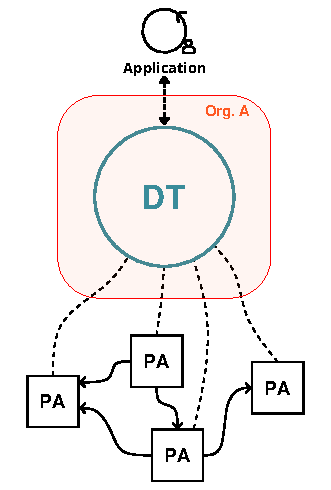
\includegraphics[width=\textwidth]{figures/hwodt/ecosystems_types-monolithic.pdf}
        \caption{\textbf{Monolithic} Ecosystem}
        \label{fig:ecosystem-monolithic}
    \end{subfigure}
    \hfill
    \begin{subfigure}[t]{0.32\textwidth}
        \centering
        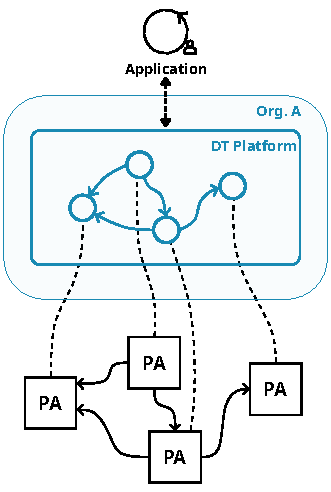
\includegraphics[width=\textwidth]{figures/hwodt/ecosystems_types-homogeneous.pdf}
        \caption{\textbf{Homogeneous} \ac{DTE}}
        \label{fig:ecosystem-homogeneous}
    \end{subfigure}
    \hfill
    \begin{subfigure}[t]{0.32\textwidth}
        \centering
        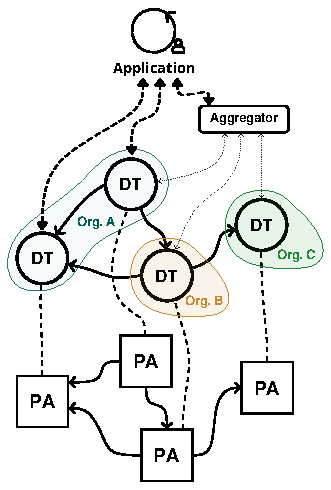
\includegraphics[width=\textwidth]{figures/hwodt/ecosystems_types-heterogeneous.pdf}
        \caption{\textbf{Heterogeneous} \ac{DTE}}
        \label{fig:ecosystem-heterogeneous}
    \end{subfigure}

    \caption{Three architectural approaches for \acp{DTE}: in \ref{fig:ecosystem-monolithic} a single \ac{DT} models the whole scenario; in \ref{fig:ecosystem-homogeneous} a single platform is used to build and deploy all the \acp{DT} in the ecosystem; in \ref{fig:ecosystem-heterogeneous} maximum flexibility is allowed, possibly reusing existing \acp{DT} under a common interface.}
    \label{fig:ecosystem-types}
\end{figure}


The characteristics and functional requirements identified for \acp{DTE} lead to different trade-offs concerning
\begin{inlinelist}
    \item the ability to evolve to accommodate changes in the domain of interest,
    \item loose coupling of the member \acp{DT}, 
    and
    \item implementation of the ecosystem functionalities.
\end{inlinelist}
%
These are discussed in this section, presenting three architectural approaches emerging from the state of the art of \ac{DTE} research and technologies (\Cref{fig:ecosystem-types}).

\subsubsection{Monolithic Ecosystem}
\label{sssec:monolithic}

The most straightforward approach is to model the entire targeted context as a single, monolithic \ac{DT}.
Due to the fuzzy definition of a \ac{PA}, even complex entities (e.g., an entire city) can serve as valid physical counterparts of a single \ac{DT}, with some models explicitly capturing multiple internal components of such entities. Examples of monolithic \acp{DT} include modeling a single \ac{DT} for entire roads~\cite{KUSIC2023101858}, hospital buildings~\cite{Peng_Zhang_Yu_Xu_Gao_2020}, or smart grids~\cite{9449682}.

The main benefit of this approach is its simplicity in deriving the overall system architecture:
all physical-world data can flow into a single system built with a consistent technological stack (\Cref{fig:ecosystem-monolithic}).
%
A monolithic \ac{DT} also offers strong modeling capabilities and facilitates services such as running simulations on a single model of the entire ecosystem.

The drawbacks of the approach are on the management side. 
Representing dynamic scenarios involving multiple heterogeneous assets with high fidelity can be challenging, and even minor updates---such as adding new entities or modifying the behavior of existing ones---may require modifying the entire \ac{DT}.
%
This approach is not suited for rapidly evolving ecosystems or contexts involving multiple stakeholders.
%
Relying on a single \ac{DT} limits technological diversity, forcing the creation of a new, unified model.


\subsubsection{Homogeneous \ac{DTE}}
\label{sssec:homogeneous}

A \ac{DTE} can be considered a \emph{Homogeneous} \acp{DTE} when the approach relies on a general-purpose platform that natively supports the definition of multiple \acp{DT} (\Cref{fig:ecosystem-homogeneous}).
%
The \acp{DT} are hence homogeneous in their modeling and implementing technology as they are created within the same platform.
%
The native support for \acp{DTE} enhances adaptability to the evolving physical world as it is simple to add and remove \acp{DT} or update models.
%
Furthermore, the modeling and technological homogeneity make implementing ecosystem services relatively easy, as in the \emph{monolithic} approach.
%
Differently, though, it is possible to highlight the individuality of the involved entities and their corresponding \acp{DT}, which may independently process the relative data flows, offering better decomposition and separation of concerns.

The dependency on a single platform, however, may introduce vendor lock-in, modeling and organizational constraints.
%
An example of this approach is the \azureTwin{} platform, which introduced the concept of a \emph{Twin Graph}\footnote{\url{https://learn.microsoft.com/en-us/azure/digital-twins/concepts-twins-graph}}
to explicitly represent relationships among \acp{DT} modeled using a uniform \ac{DTDL}.


\subsubsection{Heterogeneous \ac{DTE}}
\label{sssec:heterogeneous}

The third approach is based on introducing a common interoperability layer on top of technologically heterogeneous \acp{DT}.
%
This approach enables the reuse of existing \acp{DT} while ensuring uniform access and navigation for consumers (\Cref{fig:ecosystem-heterogeneous}).
%
\acp{DT} are implemented as standalone software components, each with specific models and technologies, and each exposing interfaces that can be used by applications directly or through intermediary aggregators.

This approach is well-suited for dynamic, open \acp{DTE} where \acp{DT} are developed by various stakeholders since the individual components are loosely coupled.
%
Furthermore, \acp{DT} are not limited to being part of only one ecosystem, granting an additional degree of flexibility.

To maintain interoperability, though, each \ac{DT} must be mapped to a shared metamodel to represent it within the ecosystem and expose a shared interface to enable seamless interaction.
This can lead to a potential loss of information and expressivity, as with any model conversion.
However, direct access to the original \ac{DT} remains possible when needing to use specialized services not easily mapped in the shared model.

Compared to the previous approaches, where ecosystem functionalities can be directly supported by the implementing technology/platform and benefit from modeling uniformity, implementing ecosystem services in heterogeneous \acp{DTE} is inherently more complex.
%
This can be achieved through either fully distributed techniques---such as polystores~\cite{dggan2015polystore} or federated and link-traversal queries \cite{schwarte2011semweb,quilitz2008querydistributed,bogaerts2021linktraversalquery}---or by introducing a middleware (as shown in \Cref{fig:ecosystem-heterogeneous}) aggregating \acp{DT} and implementing the required functionalities.
%
This doubles as a way to set a clear boundary for operations, allowing a clear definition of which \acp{DT} belong to an ecosystem.


% To make a parallel with open Web-based ecosystems, this would be similar to a web service exposing a well-documented public HTTP API, which does not prevent specialized consumers from using remote method invocation if they have specialized knowledge on how to interact with the server.

% For the approach to be successful and encourage \ac{DT} developers to join heterogeneous ecosystems, the entry barrier needs to be set at a relatively low level to ensure take-up, while still maintaining a sufficient level of complexity to meet the overall objectives~\cite{kendall2021ndt}.


%======================================================
\section{Heterogeneity and Trade-offs}
\label{sec:dte:dte:heterogeneity}
%======================================================


\begin{table}[ht]
    \centering
    \footnotesize
    \renewcommand{\arraystretch}{1.1}
    \begin{tabularx}{\textwidth}{p{3cm}|X}
    \toprule
    \midrule
    \textbf{Heterogeneity \newline Dimension} & \textbf{Description} \\
    \hline
    \hline
    Organization &
    \acp{DTE} may digitalize large-scale contexts involving \acp{PA} that belong to different stakeholders and organizations that may need to collaborate~\cite{tripathi2024infsof}
    \\
    \hline
    Domain & 
    \acp{DTE} may include assets from different application domains and hence require the integration of different domain vocabularies such as in the case of a smart city ecosystem that may span across the energy, mobility, ecology, and financial domains~\cite{Deng_Zhang_Shen_2021}
    \\
    \hline
    Purpose &
    The \ac{DT} paradigm is employed for a variety of purposes~\cite{bulter2018geminiprinciples} leading to very different \acp{DT} having to coexist in an ecosystem. Examples range from monitoring to simulation, what-if analysis, and planning.
    \\
    \hline
    Modeling &
    \ac{DT} models may vary based on the nature of the corresponding \acp{PA} with one \ac{DT} possibly having more than one model within itself~\cite{qi2021enablingtechdt}.
    For example, while a manufactured product may be effectively represented with a three-dimensional model, using differential equations may be more suited for a physics system~\cite{bulter2018geminiprinciples}
    \\
    \hline
    Technology &
    The spread of the \ac{DT} paradigm led to a variety of supporting technologies~\cite{qi2021enablingtechdt}, often creating closed vertical technological silos~\cite{Damjanovic-Behrendt_Behrendt_2019}. In complex real-world contexts where legacy is the norm, it is natural to assume that different technological stacks may coexist in the same \ac{DTE}
    \\
    \hline
    \bottomrule
    \end{tabularx}
     \caption{Dimensions of \ac{DT} heterogeneity that characterize DT ecosystems.}
    \label{tab:heterogeneity}
\end{table}


The trade-offs in the different approaches to engineer \acp{DTE} arise from the necessity of managing several \acp{DT} as a cohesive system. 
%
In general, the set of \acp{DT} belonging to the same ecosystem may be \emph{heterogeneous} for various reasons.
To better characterize this heterogeneity, it is possible to extract and analyze a set of orthogonal dimensions along which \acp{DT} may differ.

\Cref{tab:heterogeneity} briefly reports the identified dimensions through an analysis of the relevant literature on \acp{DTE}.
%
Findings demonstrate that \acp{DTE} are usually envisioned in contexts that either involve multiple stakeholders (\emph{organization dimension}) and a diverse set of assets (\emph{domain dimension}) that may require different techniques to be described effectively (\emph{modeling dimension}).
Furthermore, \acp{DT} are employed for a variety of use cases, ranging from monitoring to simulation and forecasting (\emph{purpose dimension}).
%
All these factors naturally result in technological fragmentation (\emph{technology dimension}), which is particularly evident in the current \ac{DT} technology landscape
with solutions either tailored to specific application domains~\cite{Damjanovic-Behrendt_Behrendt_2019}, or providing a general-purpose platform for handling different \acp{DT}.

As an additional factor of complexity, different stakeholders may be interested in different views of the same \ac{PA}, ending up independently developing multiple \acp{DT} to fulfill distinct business goals~\cite{dt-IoT-context-Minerva-2020}.
%
Ecosystems can then either serve a unifying purpose, connecting different views of the same \ac{PA}, or exist in parallel to serve specific perspectives of the same domain.

Heterogeneity influences the design of \acp{DTE}.
%
Namely, monolithic and homogeneous ecosystems work best when \acp{DT} are aligned for what concerns the organization and modeling dimensions, as it might be easier to align the development to common guidelines.
%
Differently, ecosystems involving multiple stakeholders, and spanning across different application domains, might require additional degrees of flexibility that only a heterogeneous approach can grant.
%
Such flexibility comes at a price: implementing ecosystem services is easier---and possibly even supported by off-the-shelf solutions---when dealing with a homogeneous set of entities. 
%
Heterogeneous \acp{DTE} must instead rely on a carefully designed interoperability layer, adapting different \acp{DT} to a common interface.


%======================================================
\section{Challenges of \aclp{DTE}}
\label{sec:dte:dte:challenges}
%======================================================

As outlined in the previous section, due to its multi-dimensional nature, heterogeneity should be regarded as an inherent source of complexity in \acp{DTE} that can not always be avoided.
%
This work focuses on addressing the challenges that arise when dealing with heterogeneous \acp{DTE}, as they represent the most general and challenging case for what concerns the design of ecosystem functionalities and the integration of existing \acp{DT} infrastructures.

Two main challenges are identified and explored in the following chapters:

\begin{itemize}
    \item \textbf{Interoperability of Heterogeneous \aclp{DT}}: enabling interaction across \acp{DT} built using different technologies, models, and purposes. This includes defining a common metamodel to represent \acp{DT} within the ecosystem and implementing mechanisms to translate between different \acp{DT} interfaces and the shared interface exposed by the ecosystem.
    %
    Addressing this challenge will answer \ref{rq:2}, with a proposal for the engineering of heterogeneous \acp{DT} as discussed in \Cref{chap:dte:hwodt}.

    \item \textbf{Deployment and Runtime Management of \aclp{DTE}}: orchestrating the deployment, configuration, and management of \acp{DT} within the ecosystem. This involves handling the dynamic nature of \acp{DTE}, including adding and removing \acp{DT} in a complex cyber-physical infrastructure. Addressing this challenge will answer \ref{rq:3}, with a proposal for the runtime management of heterogeneous \acp{DT} as discussed in \Cref{chap:dte:dtc}.
\end{itemize}

There are other significant challenges in the context of \acp{DTE} which are not directly addressed in this thesis.

These include aspects such as security and privacy, trust and governance between multiple stakeholders.
%
Although it is true that building \acp{DTE} can be effective even when considering a focused application use case with limited stakeholders, open \acp{DTE} spanning across multiple organizations can support novel forms of collaboration and value creation~\cite{kendall2021ndt}.
%
Addressing these challenges requires a broader sociotechnical perspective, that involves pushing towards open data and open standards to foster collaboration and interoperability at a larger scale~\cite{Acharya_Khan_Päivärinta_2024}.

